\subsection{Stolon}

\begin{figure}[ht!]
  \center{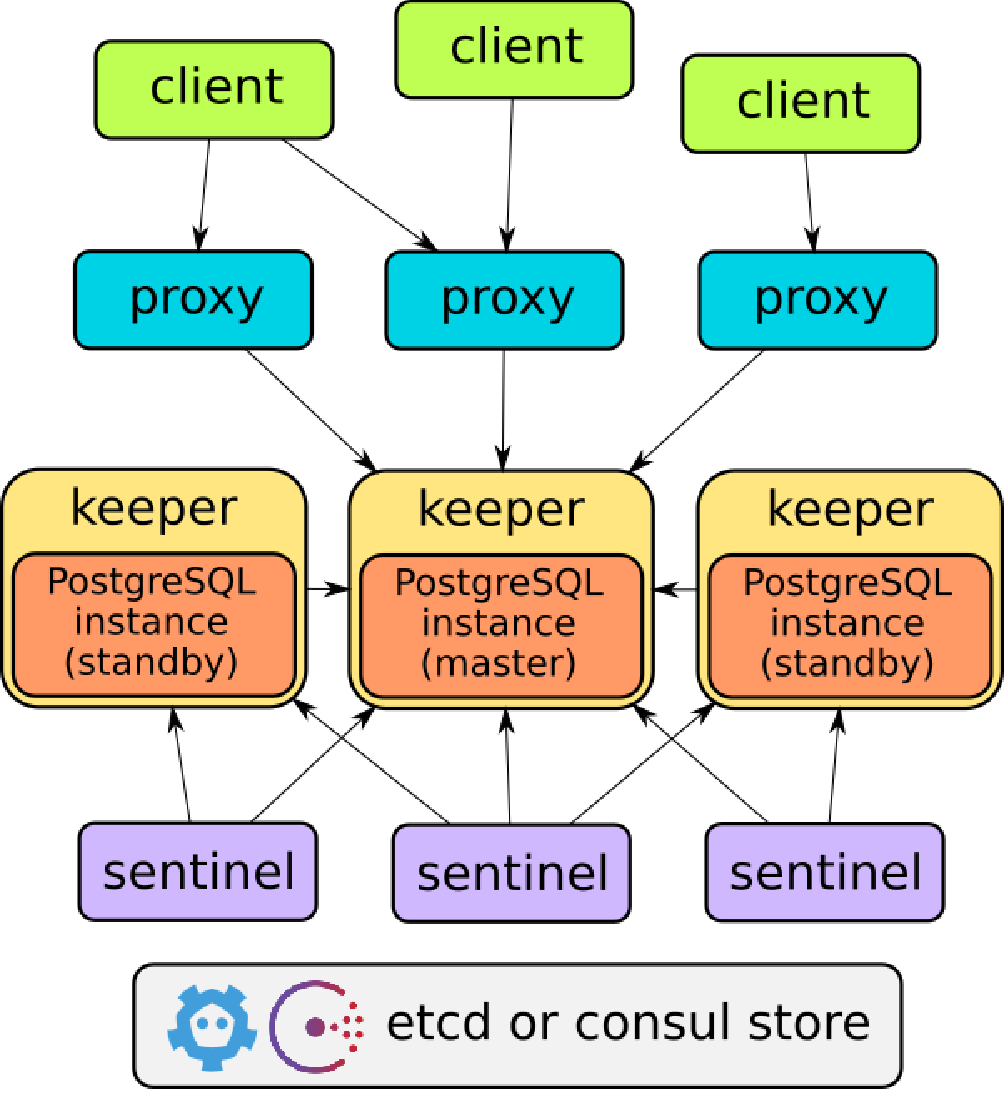
\includegraphics[width=1\textwidth]{stolon_arch.pdf}}
  \caption{Stolon архитектура}
  \label{fig:stolon_arch}
\end{figure}

\href{https://github.com/sorintlab/stolon}{Stolon}~--- это демон на Go, позволяющий автоматически обслуживать кластеры PostgreSQL с потоковой репликацией.

Особенности:

\begin{itemize}
  \item Использует потоковую PostgreSQL репликацию (асинхронная и синхронная репликация);
  \item Интеграция с \href{https://kubernetes.io/}{Kubernetes};
  \item Поддержания актуальности кластера и выборов мастера используются распределенные \href{https://en.wikipedia.org/wiki/Distributed_control_system}{DCS} хранилища (поддерживаются \href{https://coreos.com/etcd}{Etcd} или \href{https://www.consul.io/}{Consul});
  \item Автоматическое <<service discovery>> и динамическая реконфигурация кластера;
  \item Состояние кластера можно получить как запросами в DCS, так и через \lstinline!stolonctl! клиент;
\end{itemize}

Stolon состоит из 3 основных компонентов:

\begin{itemize}
  \item keeper (хранитель): управляет экземпляром PostgreSQL;
  \item sentinel: обнаруживает и контролирует keeper-ров и вычисляет оптимальное состояние кластера;
  \item proxy: точка доступа клиента, обеспечивает подключение к верному PostgreSQL мастеру в кластере;
\end{itemize}

Информация по настройке и использованию Stolon находится в \href{https://github.com/sorintlab/stolon/blob/master/doc/README.md}{официальной документации} проекта.
